\section{Flexible User Roles}
\label{sec:agile_roles}
The roles we grant users in our application are hard-coded into our application and not the permissions graded by the role.
If the \hdesk[] should be implemented at different environments, the role system would need to be more flexible. 
It is not given that all workplaces make use of the three predefined roles, therefore a more flexible role system would be needed in order to make the application more efficient and make the application more flexible as a whole.
It should also be possible to create custom user-roles with custom names.
This can be improved by introducing a double layered role system.  
This work by making a role for each controller or even the methods within the controller, then adding a high level role set which can access the low level roles. 
This allow for agile changing the privileges for an entire group of users. 
E.g. if the user of the application wants to allow clients to see statistics this can easily be changed with this improvement. An example of this alternative role system can be seen on figure \ref{fig:improved_role_system}.

\paragraph{Pros} are that the application allows more specific configuration. 
\paragraph{Cons} are the time it takes to implement it.
\paragraph{We did not implement this feature because} we realized too late that the functionality was missing, thus we did not have time to implement it.

\begin{figure}
\begin{center}
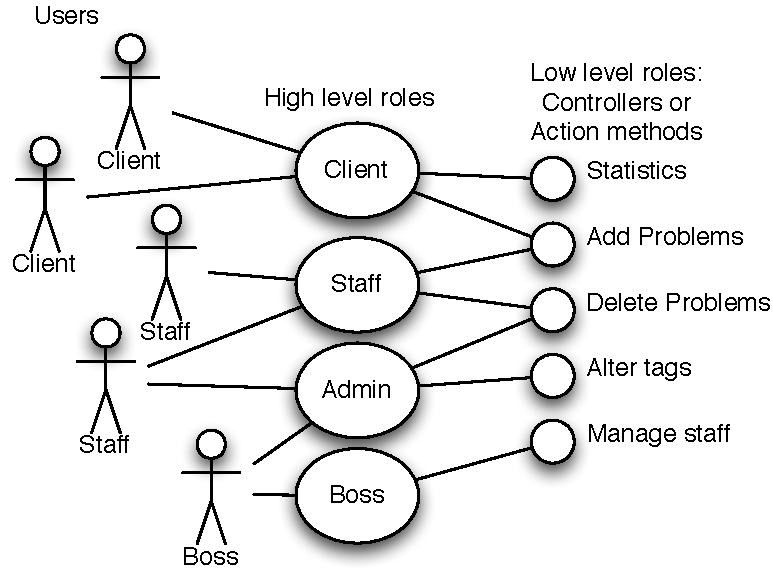
\includegraphics[scale=1]{input/epilogue/improvements/improved_role_system.pdf}
\morscaption{Example of how the roles can be structured with an improved role system}
\label{fig:improved_role_system}
\end{center}
\end{figure}
